\documentclass[10pt,letterpaper]{article}
\usepackage[utf8]{inputenc}
\title{EV 1.5 CARACTERISTICAS DE LOS CONVERTIDORES DE POTENCIA CA-CD, CD-CA, CA-CA Y CD-CD}
\author{Ascencio De Leon Agustin}
\usepackage[spanish]{babel}
\usepackage{graphicx}
\graphicspath{{imagenes/}}
\usepackage[left=2.5cm,top=2.5cm,bottom=3cm,right=2.5cm]{geometry}

\begin{document}
\maketitle
\begin{figure}[h!]
\centering
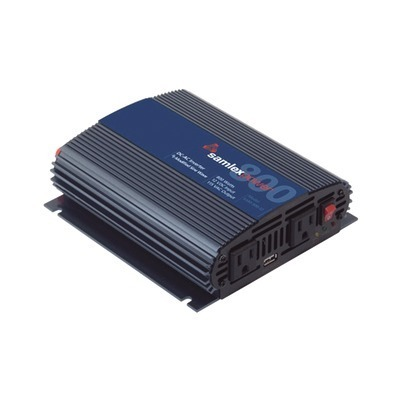
\includegraphics[scale=.9]{cacD}
\end{figure}
\newpage


CONVERTIDORES DE POTENCIA CD-CA:
Los  convertidores  de  corriente  directa  a  corriente  alterna  son  utilizados  como  drivers  de  motores  y  como  fuentes  de  corriente  alterna  ininterrumpida  y  tienen  como  objetivo  producir  una  señal  de  corriente  alterna  sinusoidal,  cuya  magnitud  y  frecuencia  puedan  ser  controladas 
\begin{figure}[h!]
\centering
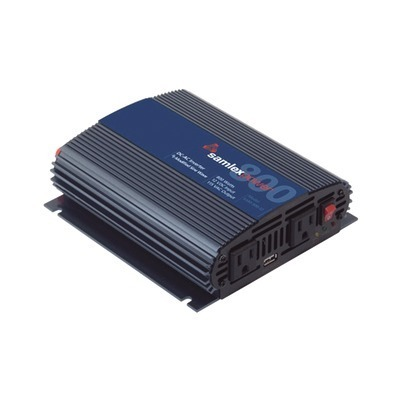
\includegraphics[scale=.8]{cacD}
\end{figure}
\newpage
CONVERTIDORES CA-CD:
Un convertidor se puede utilizar para elevar un voltaje de CD. Cuando el interruptor Q se cierra durante un tiempo t1, la corriente del interruptor se eleva la energía se almacena en un inductor L.
Si durante el tiempo t2 el interruptor se abre, la energía almacenada de inductor se transfiere a la carga a través del diodo D y la corriente del inductor se abate.
\begin{figure}[h!]
\centering
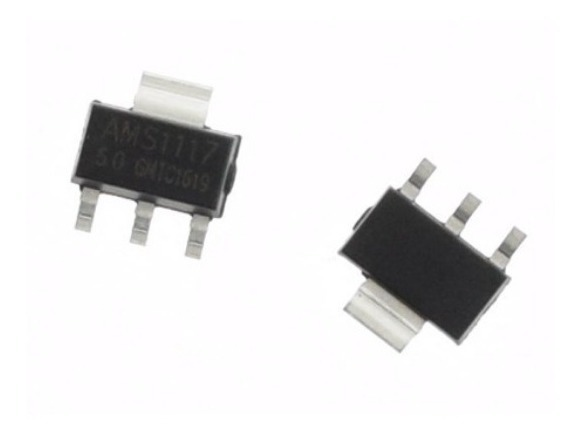
\includegraphics[scale=.5]{cacd}
\end{figure}
\newpage
CONVERTIDORES CA-CA:
•Realizan  la conversión  AC/AC  de  forma  directa y  sin  etapa  intermedia  descontinua.
•Los tiristores no necesitan bloqueo forzadogracias al paso natural por cero de la intensidad.
•Proporcionan  una  tensión  de frecuencia fundamental menor  o  igual que  la frecuencia de la tensión de entrada.
•Proporcionan una tensión con un ciertocontenido de armónicos.
\begin{figure}[h!]
\centering
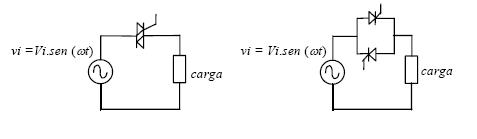
\includegraphics[scale=4]{caca}
\end{figure}
\newpage
CONVERTIDORES CD-CD:
Los convertidores CD-CD se utilizan  ampliamente en el control de los motores de tracción de automóviles eléctricos, tranvías eléctricos, grúas marinas, montacargas y elevadores de minas. En lo que a nosotros nos concierne el convertidor CD-CD se utilizará en la primera etapa del balastro  para  la  corrección  del  factor  de  potencia  y  obtener  una  salida  en  CD  estable  para  alimentar  el  inversor  resonante  el  cual  trabajará  en  alta  frecuencia.  En  este  capítulo  se  analizarán  3  topologías  de  convertidores  CD-CD  las  cuales  son:  Topología  Elevadora,  Reductora-elevadora y Flyback
\begin{figure}[h!]
\centering
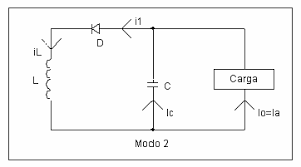
\includegraphics[scale=.9]{cdcd} 
\end{figure}
\end{document}
